\documentclass{standalone}
\usepackage{graphicx}	
\usepackage{amssymb, amsmath, amsthm}
\usepackage{color}

\usepackage{tikz}
\usetikzlibrary{calc, math}

\definecolor{light}{RGB}{220, 188, 188}
\definecolor{mid}{RGB}{185, 124, 124}
\definecolor{dark}{RGB}{143, 39, 39}
\definecolor{darker}{RGB}{124, 0, 0}
\definecolor{highlight}{RGB}{180, 31, 180}
\definecolor{darkteal}{RGB}{29, 79, 79}
\definecolor{darkolive}{RGB}{97, 123, 45}
\definecolor{gray10}{gray}{0.1}
\definecolor{gray20}{gray}{0.2}
\definecolor{gray30}{gray}{0.3}
\definecolor{gray40}{gray}{0.4}
\definecolor{gray60}{gray}{0.6}
\definecolor{gray70}{gray}{0.7}
\definecolor{gray80}{gray}{0.8}
\definecolor{gray90}{gray}{0.9}
\definecolor{gray95}{gray}{0.95}

% #1: x0
% #2: y0
% #3: R
% #4: dx
% #5: dy
\newcommand{\randpoints}[5]{
  ({#1 + #4 * (1 + 0.2 * rand) * #3 * (-1)},      {#2 + #5 * (1 + 0.2 * rand) * #3 * (0)})
  ({#1 + #4 * (1 + 0.2 * rand) * #3 * (-0.7071)}, {#2 + #5 * (1 + 0.2 * rand) * #3 * (+0.7071)})
  ({#1 + #4 * (1 + 0.2 * rand) * #3 * (0)},       {#2 + #5 * (1 + 0.2 * rand) * #3 * (+1)})
  ({#1 + #4 * (1 + 0.2 * rand) * #3 * (+0.7071)}, {#2 + #5 * (1 + 0.2 * rand) * #3 * (+0.7071)})
  ({#1 + #4 * (1 + 0.2 * rand) * #3 * (+1)},      {#2 + #5 * (1 + 0.2 * rand) * #3 * (0)})
  ({#1 + #4 * (1 + 0.2 * rand) * #3 * (+0.7071)}, {#2 + #5 * (1 + 0.2 * rand) * #3 * (-0.7071)})
  ({#1 + #4 * (1 + 0.2 * rand) * #3 * (0)},       {#2 + #5 * (1 + 0.2 * rand) * #3 * (-1)})
  ({#1 + #4 * (1 + 0.2 * rand) * #3 * (-0.7071)}, {#2 + #5 * (1 + 0.2 * rand) * #3 * (-0.7071)})
}

\pgfmathsetseed{12}
 
\begin{document}

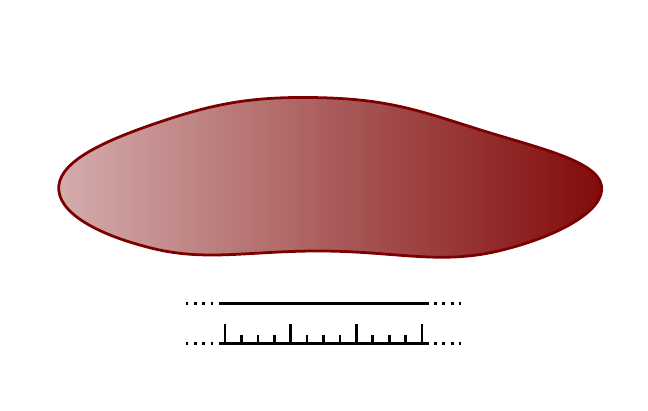
\begin{tikzpicture}[scale=1.0]
  
  \draw[white] (-3.75, -2.5) rectangle (3.75, 2);

  \pgfmathsetmacro{\dx}{2}
  \pgfmathsetmacro{\dy}{1}

  \begin{scope}
    \pgfmathsetseed{12}
    \clip plot [smooth cycle, tension=0.75] coordinates { \randpoints{0}{0}{1}{1.5 * \dx}{1 * \dy} } -- cycle;
    \foreach \n in {0, 1, ..., 150} {
    \pgfmathsetmacro{\x}{2 * (\n / 75 - 1)}
    \pgfmathsetmacro{\prop}{100 * \n / 150}
    \colorlet{custom}{darker!\prop!light};
    \draw[custom, line width=1.75] (\dx * \x, -1) -- (\dx * \x, +1.25);
  }
  \end{scope}
  
  \pgfmathsetseed{12}
  \draw[darker, line width=1]
    plot [smooth cycle, tension=0.75] coordinates { \randpoints{0}{0}{1}{1.5 * \dx}{1 * \dy} } -- cycle;
  
  
  \pgfmathsetmacro{\rdx}{1}
  \pgfmathsetmacro{\rdy}{1}
  \draw[line width=1] (-1.3 * \rdx, -1.5 * \rdy) -- (+1.3 * \rdx, -1.5 * \rdy);
  \draw[line width=1, dotted] (-1.75 * \rdx, -1.5 * \rdy) -- (-1.3 * \rdx, -1.5 * \rdy);
  \draw[line width=1, dotted] (+1.3 * \rdx, -1.5 * \rdy) -- (+1.75 * \rdx, -1.5 * \rdy);

  \draw[line width=1] (-1.3 * \rdx, -2 * \rdy) -- (+1.3 * \rdx, -2 * \rdy);
  \draw[line width=1, dotted] (-1.75 * \rdx, -2 * \rdy) -- (-1.3 * \rdx, -2 * \rdy);
  \draw[line width=1, dotted] (+1.3 * \rdx, -2 * \rdy) -- (+1.75 * \rdx, -2 * \rdy);
  
  \foreach \x in {-6, -5, ..., 6} {
    \draw[line width=1] (\rdx * \x * 1.25 / 6, -2) -- +(0, 0.1);
  }
  
  \foreach \x in {-6, -2, ..., 6} {
    \draw[line width=1] (\rdx * \x * 1.25 / 6, -2) -- +(0, 0.25);
  }
  
\end{tikzpicture}

\end{document}  